\documentclass[twocolumn,a4paper,10pt]{scrartcl}

\usepackage[T1]{fontenc}
\usepackage[latin1]{inputenc}
\usepackage[paper=a4paper,left=16mm,right=16mm,top=20mm,bottom=25mm]{geometry}
\usepackage{times}
\usepackage{graphicx}
\usepackage{fancyhdr}
\usepackage{fancybox}
\usepackage[round]{natbib}
\usepackage[labelfont=bf]{caption}
\usepackage{bm}
\usepackage{natbib}
\usepackage{hyperref}
\usepackage{tikz}
\bibliographystyle{apalike}
\renewcommand{\headrulewidth}{0.0pt}
\pagestyle{fancy} \setlength{\headheight}{21pt}
\lhead{\parbox[t]{2cm}{\textbf{\normalsize }}\\} 
\rhead{\small{\sffamily $\mathsf{11^{th}}$ International Conference on Multiphase Flow,\\ICMF 2023, Kobe, Japan, April 2--7, 2023}} \fancypagestyle{plain}

\setlength{\columnsep}{22pt}

\bibpunct{(}{)}{;}{a}{}{,}
\setlength{\bibhang}{0pt}

\addtokomafont{section}{\normalsize}

\begin{document}
\title{\vspace{-1.3cm} \sffamily \large On the phenomenology of pairwise interactions in a buoyancy driven flow. \\
\vspace{0.2cm} \small Using Nearest Particles Statistics.}
\author{\vspace{3mm} Nicolas Fintzi$^1$, Jean-Lou Pierson$^2$ and Stephane Popinet$^3$\\
% \normalsize Affiliation University, School, Department, Institute\\
% \normalsize Address, City, Postal Code, Country\\
% \normalsize E-mail\\
\normalsize $^{1, 2}$IFP Energies Nouvelles, $^3$CNRS \& Sorbonne Universite.\\
\normalsize $^{1, 2}$Rond-point de l'echangeur de Solaize, 69360 Solaize, France.\\
\normalsize $^3$4 place Jussieu, 75005 Paris, France.\\
\normalsize Nicolas.fintzi@ifpen.fr, jean-lou.pierson@ifpen.fr, popinet@basilisk.fr.\\
\tiny\\
\normalsize \textbf{Keywords}: Emulsion, droplets, population balance equations, film drainage. }
\date{}
\twocolumn[{\csname @twocolumnfalse \endcsname \maketitle

\section*{Abstract} 
The population balance equations (PBE) have been used in engineering for decades. 
However, there is a clear lack of accurate closure regarding the coalescence source term in emulsion modeling.  
Therefore, in a multiscale strategy, we perform tri-periodic simulations of buoyant emulsions.
In addition, to providing data for the closure terms appearing in the averaged models (PBE and averaged Navier-Stokes equaitons), tri-periodic simulations are of great interest to understand and describe pairwise interactions of droplets.
In this work, we present a new approach to characterize the nature of the interactions through the statistical analysis of the relative motion of pairs of particles. 
The empirical statistics, together with film drainage equations, provides us with an accurate modeling for the probability of coalescence of pairs of droplets in buoyant suspension. 
\\[12pt]
}]


\section*{Introduction}
In PBE, a source term is used to account for breakage and coalescence of the droplets. 
In this source term, we often make use of film drainage equations to determine the probability of coalesce during the time of contact of two droplets.
Additionally, we use an expression for collision frequency of droplets inside the bulk.
Together, they provide an expression for the coalescence source term. 
Those models assume a specific configuration for the bulk (e.g. turbulent, buoyant or sheared motion), and for the colliding pairs of droplets (normal or tangential collisions).
In the perspective of modeling buoyant emulsions using PBE, it is of great interest to determine the most probable collision event, and the most accurate contact time and collision frequency. 
Therefore, we used the code Basilisk (\url{http://basilisk.fr}) to perform tri-periodic simulations of buoyant emulsions. 
This code is perfectly suited for this kind of problem thanks to its strong VOF capabilities. 
Then, we analyzed the pairwise collision events using the nearest particle statistics, i.e. we define a pair by a particle and its nearest neighbor. 
This enables us to get the averaged relative and absolute characteristics of droplets pairs during a collision and deduce the nature of this interaction.  
Lastly, we show how to derive a semi empirical model (based on \citet{chesters1991modelling}) for the probability of coalesce, knowing the distribution of the characteristics of the pair (relative position, velocities \ldots) in the most likely kind of interaction. 
The averaged time of contact and contact frequency can be computed within the same simulations. 
Therefore, the last step is the development of accurate closures for the coalescence source term. 

\section*{Numerical Methods.}

To archive tri-periodic simulations, we used a square mesh for 2D cases, and a cubic multigrid for 3D ones,
inside which we initialized an array of droplets subjects to buoyancy forces only. 
The Navier-Stokes equations are discretized with a centered scheme. 
The two-phase flow solver use the Volume Of Fluid (VOF) method.
The reconstruction of the interfaces is computed using Piecewise Linear Interface Calculation (PLIC). 
Lastly, the surface forces are computed assuming a constant surface tension coefficient. 
Consequently, the solver compute the one-fluid formulation of the momentum and mass conservation equation for Newtonian fluid. 
It reads,
\begin{equation}
    \rho \frac{\partial \bm{u}}{\partial t} +\rho \bm{\nabla}\cdot(\bm{uu}) = \bm{\nabla} \cdot \bm{\sigma} + \bm{b} + \bm{f_\sigma} \delta_S,
\end{equation}
\begin{equation}
    \bm{\nabla} \cdot \bm{u} = 0,
\end{equation}
where $\delta_S$ is the surface distribution function, $\bm{f_\sigma}$ the surface force defined as the curvature times the surface tension coefficient along the normal of the droplet surface. 
$\bm{\sigma}$ is the Newtonian stress tensor and $\bm{b}$ is the body force vector such as gravitational acceleration.
\begin{figure}[h!]
    \centering
    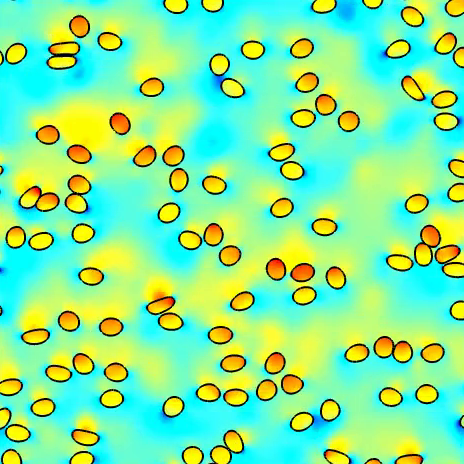
\includegraphics[width = 0.22\textwidth]{image/pic/bulles.png}
    % 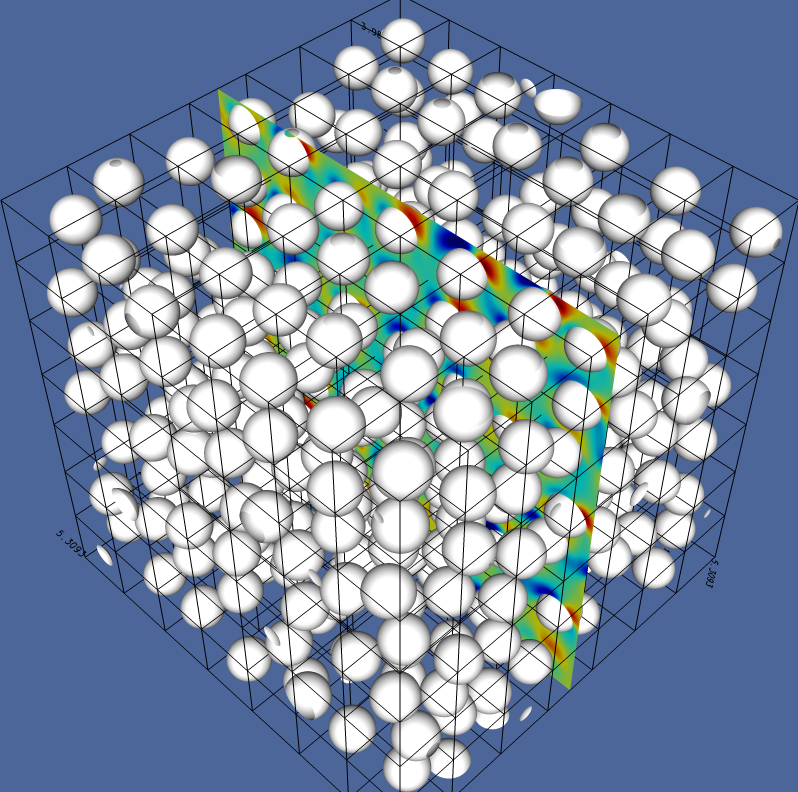
\includegraphics[width = 0.35\textwidth]{image/3D/sim49.png}
    \caption{Pressure field and interfaces of a tri-periodic simulation of buoyant droplets $Ga = 50$, $\phi = 0.15$.}
    \label{fig:pic}
\end{figure}
The main specificity of these simulations is the use of the \texttt{no-coalescence.h} header file.
This algorithm developed by \citep{mani2021numerical} prevents numerical coalesce to occur, which enable us to study a specific population of droplets within time.
Besides, we change the simulation reference frame by applying a constant acceleration on the whole domain.
This way we can carry out simulations for an arbitrary amount of time while the bulk velocity remain null. 

The physical dimensionless parameters studied are the following.
The \textit{Galileo number}, $Ga$, which is the ratio of the buoyancy forces over
the viscosity forces.
The \textit{Bond number}, $Bo$, or the ratio between the buoyancy forces and surface tension forces.
The viscosity and density ratio are respectively noted, $\mu_r$ and $\rho_r$,(ratio of the dispersed phase over the continuous phase),
and the volume fraction of the dispersed phase is noted $\phi$. 
A screenshot of the simulated pressure fields and the droplets interfaces in a typical configuration is shown figure \ref{fig:pic}.



\section*{Results and Discussion}

For a given droplet, a large amount of properties and relative properties can be computed between this droplet and its nearest neighbor. 
In this study we focused on four of them (see figure \ref{fig:droplets}). 
The relative velocity $\bm{u_{rel}}$.
The angle between the direction of contact and the horizontal  referred as $\theta$. 
The relative angle of contact $\beta$ between the direction of the relative velocity, and the direction of contact. 
And finally the distance to the closest particles $d_{nbr}$. 
\begin{figure}[h]
    \centering
    \begin{tikzpicture}[ scale = 0.9]
        \draw[fill=gray](0,0)circle (0.5);
        \draw[fill=gray](3,1)circle (0.5);
        % \draw[fill=gray,opacity=0.2](5,-0.2)circle (0.5);
        % \draw[fill=gray,opacity=0.2](-3,2)circle (0.5);
        % \draw[fill=gray,opacity=0.2](-5,0.2)circle (0.5);
        \draw[dashed](0,0)--(3,1)node[midway,above left]{$\bm{d}_{nbr}$};
        \draw[very thick,<-,blue](-1,0)--++(0,1)node[right]{$\bm{b}$};
        \draw[very thick,->,red](3,1)--++(-1.5,0.5)node[above left]{$\bm{U_{rel}}$};
        \draw[very thick,->](0,0)--++(1,0)node[below right]{$\bm{e_x}$};
        \draw[very thick,->](0,0)--++(0,1)node[left]{$\bm{e_y}$};
        \draw(3,1)++(199:1)node[above left]{$\beta$} arc(199:159:1);
        \draw(0,0)++(0:1)node[above right]{$\theta$} arc(0:20:1);
    \end{tikzpicture} 
    \caption{Scheme of the relative parameters between a droplet and its nearest neighbor.}
    \label{fig:droplets}
\end{figure}
Then, by taking a sample of particles pairs large enough, it is possible to derive an empirical probability density function, $P(\theta,\beta,d_{nbr},u_{rel})$, (inspired from kinetic theory pair distribution functions).
This probability density function is implicitly dependent on the dimensionless parameters $Ga$, $Bo$, $\phi$,$\mu_r$ and $\rho_r$.

\begin{figure}
    \centering
    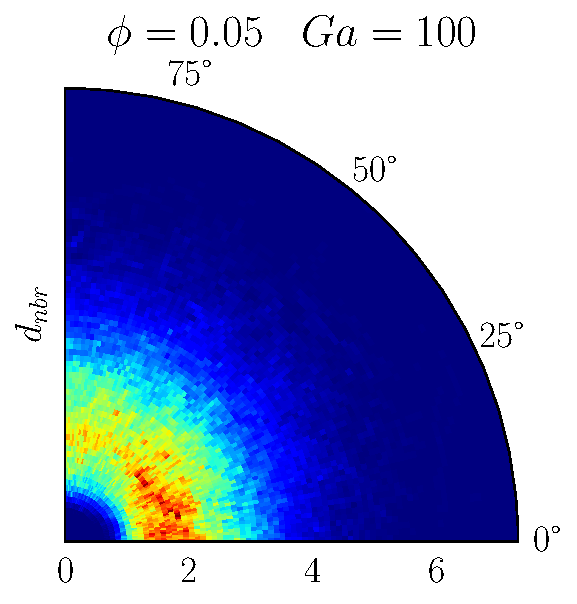
\includegraphics[width =0.19\textwidth]{image/N_10/beta/2DMAP_theta_distmin_dmin_10_Bo1PHI0_05mu_r0_42Ga100.pdf}
    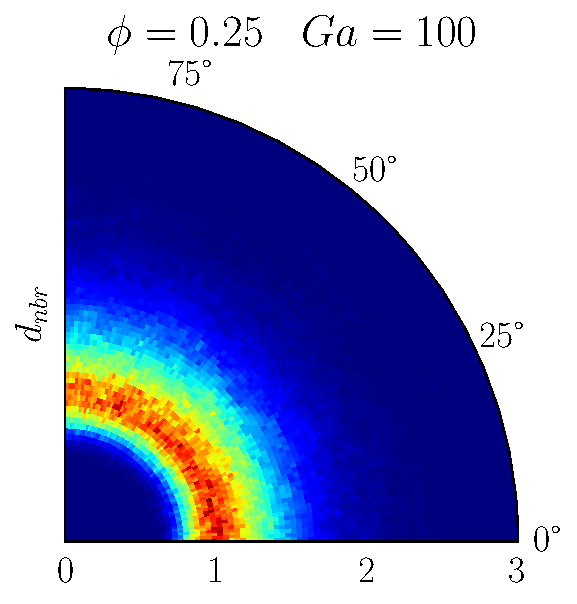
\includegraphics[width =0.19\textwidth]{image/N_10/beta/2DMAP_theta_distmin_dmin_10_Bo1PHI0_25mu_r0_42Ga100.pdf}
    \caption{Radial distribution function of the nearest particle $P(\theta,d_{nrb})$ for $\phi=0.05$ and $\phi=0.25$.}
    \label{fig:icmf}
\end{figure}
As an example, figure \ref{fig:icmf} shows the reduced probability density function $P(\theta,d_{nbr})$ in a polar plot representation.
From which we can deduce that the collisions are more likely to occur horizontally in a dilute suspension, while it is rather isotropic in a dense suspension. 
This phenomenon is already widely known in the literature.
% The study of the other properties permitted us to conclude on the average behavior of collisions depending on the physical parameters. 
By studying the distribution $P(d_{nbr})$, we found out that the interaction between the particles and their nearest neighbor is in average at close contact for high $Ga$, $\phi$ and $Bo$, whereas at low $Ga$,$\phi$ and $Bo$ the interaction occurs at longer distance. 
Another observation shows that the interactions between pair of particles are in average tangential interactions (i.e. $\beta \approx \pi/2$). 
In addition, the closer the particles get to each other, the higher the probability of having a tangential interaction is. 
This means that all the models of film drainage considering a normal approach (which is the case of most of them) are inaccurate in buoyant emulsions where the contact are more likely to be tangential. 
Therefore, to account for these facts, we add a weighing function based on the distribution $P(\theta,\beta,d_{nbr},u_{rel})$, to the classic probability of coalesce model based on the film drainage equations. 
This way, we are able to accurately model the probability of coalesce term. 
Then, together with the empirical expression of the averaged time of contact, and the averaged collision frequency, we are able to predict the coalescence source term of the PBE. 

\section*{Conclusion}

In this work, we bring strong evidence on the nature of the pairwise interaction in buoyant emulsions. 
We show that the system is isotropic at high $\phi$ and oriented normal to the gravity for low $\phi$.
Besides, we show that the interactions are more likely to happen tangentially,
while most of the film drainage model consider normal approach. 
Therefore, in a last step, we propose semi-empirical models, based on the film drainage equations and on our empirical statistics, to describe more accurately the probability of coalescence for pairs of droplets. 
Based on these results, semi-empirical expression for the coalescence kernel will be proposed. 

In a further work we will consider bi-periodic shearing flows simulations, so that we can compute relevant semi-empirical formulas for the mean first order closure terms appearing in the PBE and in the averaged Navier-Stokes equations (stresslet and torque).

% \section*{Acknowledgments}
% Please place an optional section (if needed) before References.

\bibliography{Bib/bib_bulles.bib}
\end{document}
